\documentclass[fleqn,moreauthors,10pt]{ds_report}
\usepackage[english]{babel}
\usepackage{listings}
\usepackage{xcolor} % For custom colors
\usepackage{booktabs}
\usepackage{caption}


\definecolor{codegreen}{rgb}{0,0.6,0}
\definecolor{codegray}{rgb}{0.5,0.5,0.5}
\definecolor{codepurple}{rgb}{0.58,0,0.82}
\definecolor{backcolour}{rgb}{1, 1, 1}

\lstdefinestyle{mystyle}{
    backgroundcolor=\color{backcolour},   
    commentstyle=\color{codegreen},
    keywordstyle=\color{magenta},
    numberstyle=\tiny\color{codegray},
    stringstyle=\color{codepurple},
    basicstyle=\ttfamily\footnotesize,
    breakatwhitespace=false,         
    breaklines=true,                 
    captionpos=b,                    
    keepspaces=true,                 
    numbers=left,                    
    numbersep=5pt,                  
    showspaces=false,                
    showstringspaces=false,
    showtabs=false,                  
    tabsize=2
}
\lstset{style=mystyle}

\graphicspath{{fig/}}

\JournalInfo{FRI Natural language processing course 2025}

\Archive{Project report} 

\PaperTitle{Conversational Agent with Retrieval-Augmented Generation} 

\Authors{Katarina Velkov, Nejc Krajšek, Luka Sabotič}

\affiliation{\textit{Advisors: Aleš Žagar}}

\Keywords{Conversational agent, Retrieval-Augmented Generation}
\newcommand{\keywordname}{Keywords}

\Abstract{
abstract
}

\begin{document}

\flushbottom 

\maketitle 

\thispagestyle{empty} 

\section*{Introduction}
Large language models (LLM) rely solely on their pre-trained knowledge to generate responses. 
These models have proved to be powerful but they are prone to generating hallucinated or inaccurate information. 
Furthermore their use in specialized fields has proved to be challenging as LLMs are trained mostly on publicly available 
data and are not updated after new data arises. That is why the need for more advanced models has emerged. Retrieval-Augmented Generation (RAG) enables LLMs to 
retrieve more relevant information from various external databases and web sources during conversations. 
This process allows for more accurate, domain-specific and up-to-date responses.

The aim of this project is to build a conversational agent using the RAG technique. We will use an existing large language model, 
expand it to be able to query linked domain-specific databases. We will evaluate 
the performance of our model by comparing it to the original LLM to discover improvements our implementation brought and also other RAGs available online to inspect the overall quality of our work.


\section*{Related work}
The concept of Retrieval-Augmented Generation (RAG) was first introduced in 2020 by \cite{NEURIPS2020_6b493230}, who proposed a framework that combines the strengths of large language models (LLMs) with external knowledge retrieval. Since then, RAG has seen significant advancements, particularly in the context of domain-specific applications and conversational agents.

Since we are focusing on RAG of code and code-based answers, we also took a look at \cite{large_codebaseRAG}. The authors explain how natural language RAG differs from code-based applications. They emphasize chunking as the crucial difference and explain how it should be done to preserve context such as import statements and dependencies across all chunks of the code file. \cite{sweepai} provide open source code for their chunking algorithm and other RAG components as are used in the Jet Brains Sweep AI coding assistant. Here, the chunking algorithm differs quite a lot from the standard approach for natural language RAG. Programming itself is quite prone to syntax errors, not to mention LLM generated code. This is why \cite{self-correction} provide a RAG pipeline that performs dependency and syntax unit tests on the generated code to ensure correctness of the output, which we see as a good idea for our project.

Another relevant work is the survey titled "Retrieval-Augmented Generation for Large Language Models: A Survey," \cite{gao2024retrievalaugmentedgenerationlargelanguage}, which provides a comprehensive overview of RAG's evolution. The survey categorizes RAG into three paradigms: Naive RAG, Advanced RAG, and Modular RAG. It highlights the importance of retrieval, generation, and augmentation techniques in enhancing the performance of RAG systems. The survey also discusses the challenges and future directions of RAG, such as improving robustness, handling long contexts, and integrating multimodal data.
	


\section*{Methods}
We have developed a retrieval-augmented generation to provide relevant context to a conversational agent, which then produces the answer to the user query. We are focusing on the programming and debugging domain, trying to create a model that will correctly generate, complete and correct the given programming code and answer other programming-related questions. 

We used Stack Overflow \cite{StackOverflow} question-answer pairs as our context database, for now only  focusing on python-related content due to the computational complexity of the pipeline. Later, if resources allow, we are going to expand to other languages as well.

\subsection*{Data preparation}
As mentioned, we are using Stack Overflow data, specifically extracted python tagged questions from Google Big Query's public Stack Overflow dataset. We are not only  interested in question and answer contents, but also tags and Stack Overflow scores, for pre- and post-retrieval processing.

\subsection*{Chunking}
We split each answer-question pair into multiple chunks. For each chunk, we save the text to be embedded and also some metadata that will help at the retrieval step. For a question-answer pair, we embed: the question with the answer stored as metadata, the answer, and all the code blocks we find in answers. We don't use code from the question texts, as it often contains errors and is thus in the question body. We use a very simple code identifier function that claims something is code if it is inside '$<$code$>$' blocks, longer than 10 characters and contains at least two lines, as code usually spans across multiple lines. 

\subsection*{Embedding}
For the embedding, we are using the all-MiniLM-L6-v2 \cite{miniLM}, which embeds text into a 384-dimensional dense vector space. Embeddings are then stored in a vector database, provided by the Chroma \cite{chroma} library. It automatically embeds and stores the chunks. It also provides easy retrieval by only calling the get function with the query, distance function and the number of wanted results. 

\subsection*{Retrieval}
We retrieve context chunks by embedding the user query and returning the 10 closest results by cosine distance. For the chunks that represent questions, we return the answer instead of the question, as this is the more relevant information for the user; we want to answer their question, not repeat what they asked. Code and answers are just returned. 

\subsection*{Reranking}
After retrieval, the results are reranked using the cross encoder model bge-reranker-base \cite{reranker_model}. From the 10 retrieved results, we selected top 3 results, which are then used as context for the LLM.

\subsection*{Augmentation}
When we have both the user question and the relevant contexts, we build a prompt that will be passed to the LLM. To do this, we use the following function:
\begin{lstlisting}[language=Python]
def build_prompt(self, query, results):
    contexts = self.context_from_results(results)
    return f'''
    Answer the following code related question using the context provided inside triple qoutes in it is useful.
    In the answer provide an example of code that is related to the question.
    If you do not know the answer, say that you do not know. Do not try to invent the solution.
        

    Question: {query}


    ```{''.join(f"Context {i}: {context}{chr(10)}{chr(10)}" for i, context in enumerate(contexts))}```

        
    Answer:

    '''
\end{lstlisting}
This is a basic prompt with the most important instructions. Further prompt engineering is a subject of later work, when more important parts are finished.

\subsection*{Generation}
We chose the StableLM 2 Zephyr 1.6B \cite{stabilityAI} as our LLM. This was because it is a poorly performing model for programming and mathematics tasks and we hope for significant differences in the results between using the basic model query and our RAG injection. 
\begin{figure}[h]
    \centering
    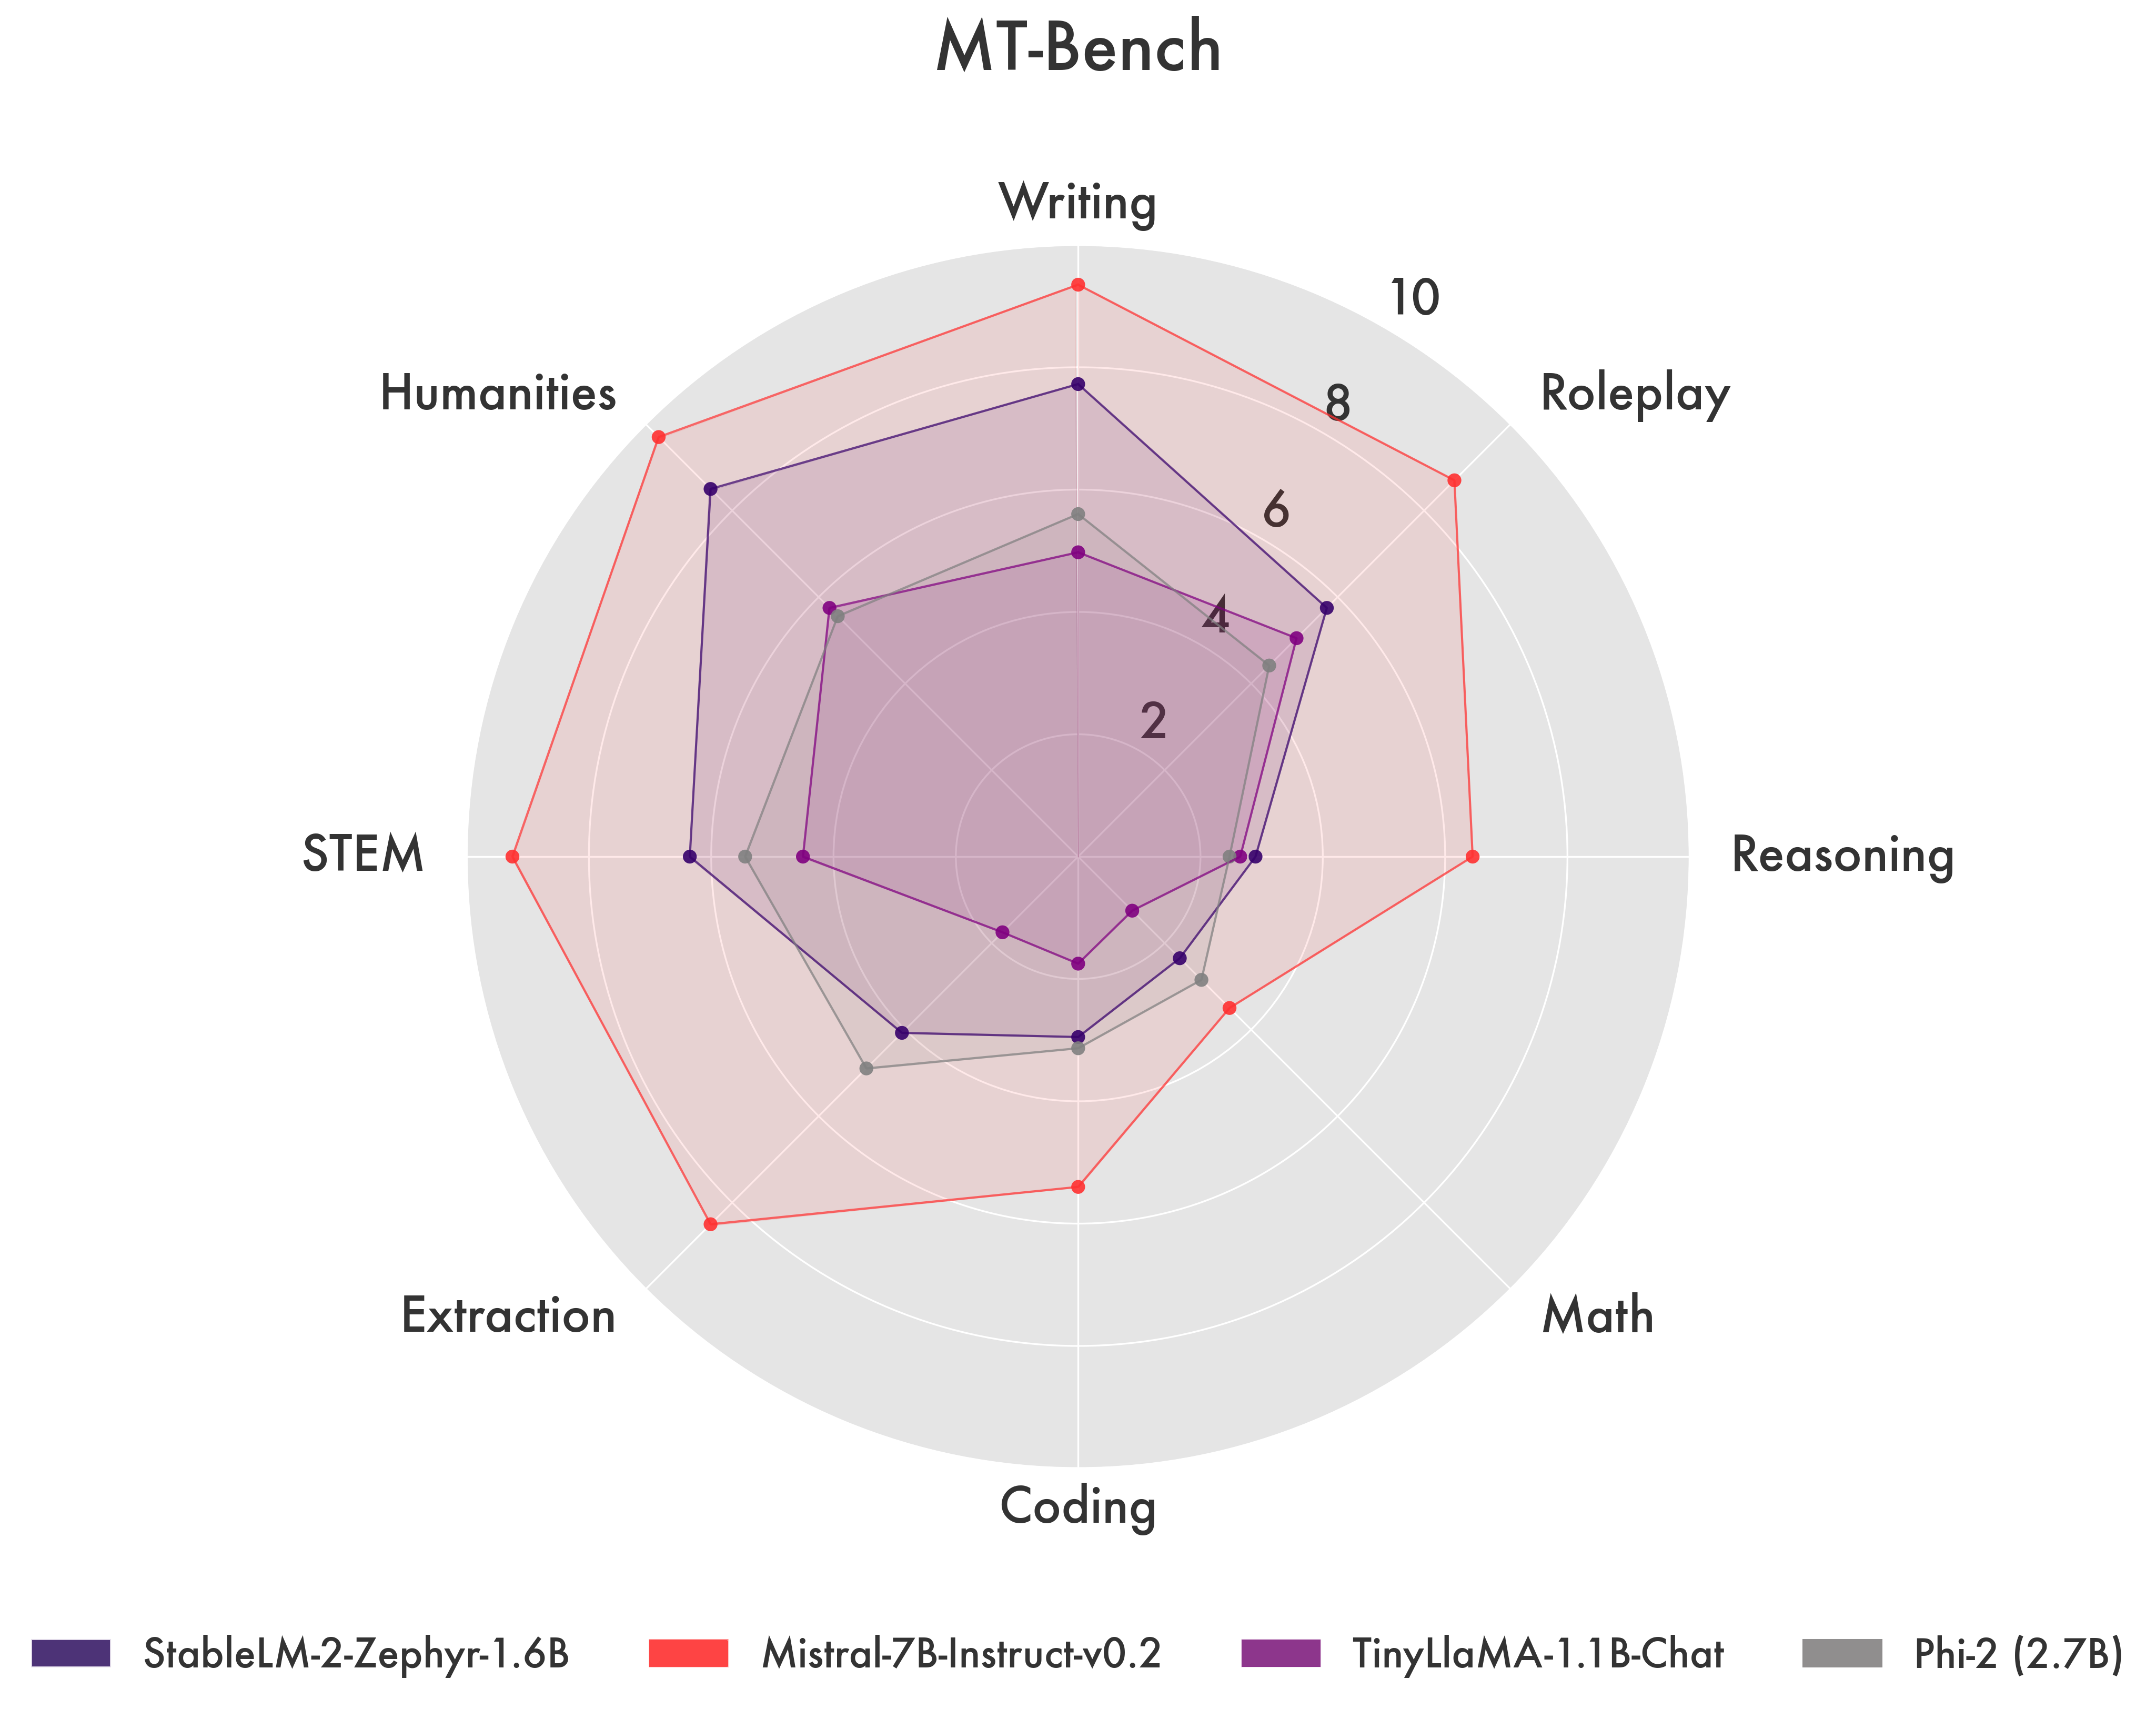
\includegraphics[width=0.8\linewidth]{fig/QH00HVM3lg-5f17U_py4K.png}
    \caption{Performance of the selected model compared to other similar-sized models.}
    \label{fig:example} % For cross-referencing
\end{figure}


The obtained answers to queries, generated using the RAG model, were then processed as to remove "Incorrect answer" parts, remove markdown (eg. ```python) and the whitespace was normalized. In the evaluation step, the answers were compared to the ground truth answers, which were processed in the same way. The results of the evaluation separately, and averaging, on the three sets are shown in the Table \ref{tab:rag_results}. 


\section*{Results}
For evaluation of our Retrieval-Augmented Generation (RAG) model for assisting with Python coding queries, we made a human evaluation and quantitative evaluation using ROUGE-1, ROUGE-L and BERTScore F1 evaluation metrics. We created three sets of queries, divided by the difficulty of the coding question/instruction. The first set consists of 14 simple questions, second of 13 semi-advanced instructions and third of 7 advanced tasks. The first set is meant to test model's ability to answer and provide code snippets on simple coding questions. The second set is meant to test the model's ability to provide more complex answers and implement specific algorithms, such as implementing a simple calculator and check for palindromes. The third set is meant to test advanced tasks, such as implementing a machine learning model. 

The following tables show the evaluation results of the RAG model across the three sets of questions, categorized by difficulty and the average results across all sets. The evaluation metrics used are ROUGE-1, ROUGE-L and BERTScore. The ROUGE-1 measures unigram overlap, the ROUGE-L is a measure of the longest common subsequence. BERTScore F1 compares the semantic similarity between the generated answer and the ground truth.

\begin{table}[h]
\centering
\caption{Evaluation results of the RAG model across different difficulty categories.}
\begin{tabular}{lccc}
\toprule
\textbf{Category} & \texttt{ROUGE-1} & \texttt{ROUGE-L} & \texttt{BERT F1} \\
\midrule
Simple         & 0.25 & 0.21 & -0.49 \\
Semi-Advanced  & 0.29 & 0.26 & -0.16 \\
Advanced       & 0.16 & 0.11 & -0.31 \\
\midrule
\textbf{Average} & \textbf{0.24} & \textbf{0.19} & \textbf{-0.32} \\
\bottomrule
\end{tabular}
\label{tab:rag_results}
\end{table}


The human evaluation results were obtained by 2 evaluators (authors), who evaluated the answers on a scale from 1 to 5, regarding 7 predetermined categories: (Answer) relevancy, Correctness, (Task) completness, Clarity, Usefulness and Conciseness. The results were then normalized to range from 0 to 1, where 0 is the worst and 1 is the best score. The results are shown in Table \ref{tab:metrics}.

\begin{table}[h]
\centering
\caption{Evaluation metrics by question complexity (normalized to [0,1])}
\small
\begin{tabular}{lccc}
\toprule
Metric & Simple & Semi-Advanced & Advanced \\
\midrule
Relevancy     & 0.58 & 0.72 & 0.51 \\
Correctness   & 0.54 & 0.61 & 0.43 \\
Completeness  & 0.52 & 0.70 & 0.45 \\
Clarity       & 0.54 & 0.67 & 0.43 \\
Usefulness    & 0.51 & 0.63 & 0.40 \\
Conciseness   & 0.57 & 0.68 & 0.49 \\
\bottomrule
\end{tabular}
\label{tab:metrics}
\end{table}




\section*{Discussion}
The developed RAG model demonstrated capabilities of providing and generating helpful code snippets. The RAG model outperforms the baseline LLM - the RAG model benefited from access to the database of coding answers from Stackoverflow. The simple and semi-advanced questions were answered with a good degree of relevancy and correctness. But we can see a clear drop in performance with the advanced instructions. The semi-advanced questions had higher ROUGE scores, possibly due to the fact that they were more specific or better represented in the database. The advanced questions were more complex and required more specific knowledge, which the model struggled with. 

The quantitative results are interestingly in alignment with the human evaluation results. Semi-advanced questions consistently score higher across all quantitative and qualitative metrics, while advanced score the lowest. The RAG model demonstrates better accuracy on mid-level questions, probably due to their more balanced complexity and clearer intent.

The ROUGE metrics show that RAG produces answers reasonably well, but the BERTScore F1 is negative (the range goes from -1 to 1 because of the cosine similarity calculation), which indicates that the answers are not very similar to the ground truth. The semantic content of the answers, which BERTScore measures, is not aligning well with the provided ground truth answers. This could be because RAG model is not able to generate answers that are very similar to the ground truth, but possibly answers more in regard to the question. 





\bibliographystyle{unsrt}
\bibliography{report}

\end{document}